\documentclass[a4paper,notitlepage]{article}
\usepackage[utf8]{inputenc} %Make sure all UTF8 characters work in the document
\usepackage{listings} %Add code sections
\usepackage{color}
\usepackage[yyyymmdd]{datetime}
\usepackage{graphicx}
\usepackage{titling}
\usepackage{titlesec}
\usepackage{listliketab}
\usepackage{longtable}
\usepackage{textcomp}
\usepackage[hyphens]{url}
\usepackage[bottom]{footmisc}
\definecolor{listinggray}{gray}{0.9}
\definecolor{lbcolor}{rgb}{0.9,0.9,0.9}
\usepackage{geometry}
\geometry{margin=3cm}
\usepackage{parskip}

\hyphenation{regres-sions-test-er}

\renewcommand{\dateseparator}{--}
\renewcommand{\arraystretch}{1.3}
\newcommand{\at}{@}
\titlespacing*\section{0pt}{10pt plus 4pt minus 2pt}{0pt plus 2pt minus 2pt}
\titlespacing*\subsection{0pt}{10pt plus 4pt minus 2pt}{0pt plus 2pt minus 2pt}
\pretitle{%
\begin{center}
	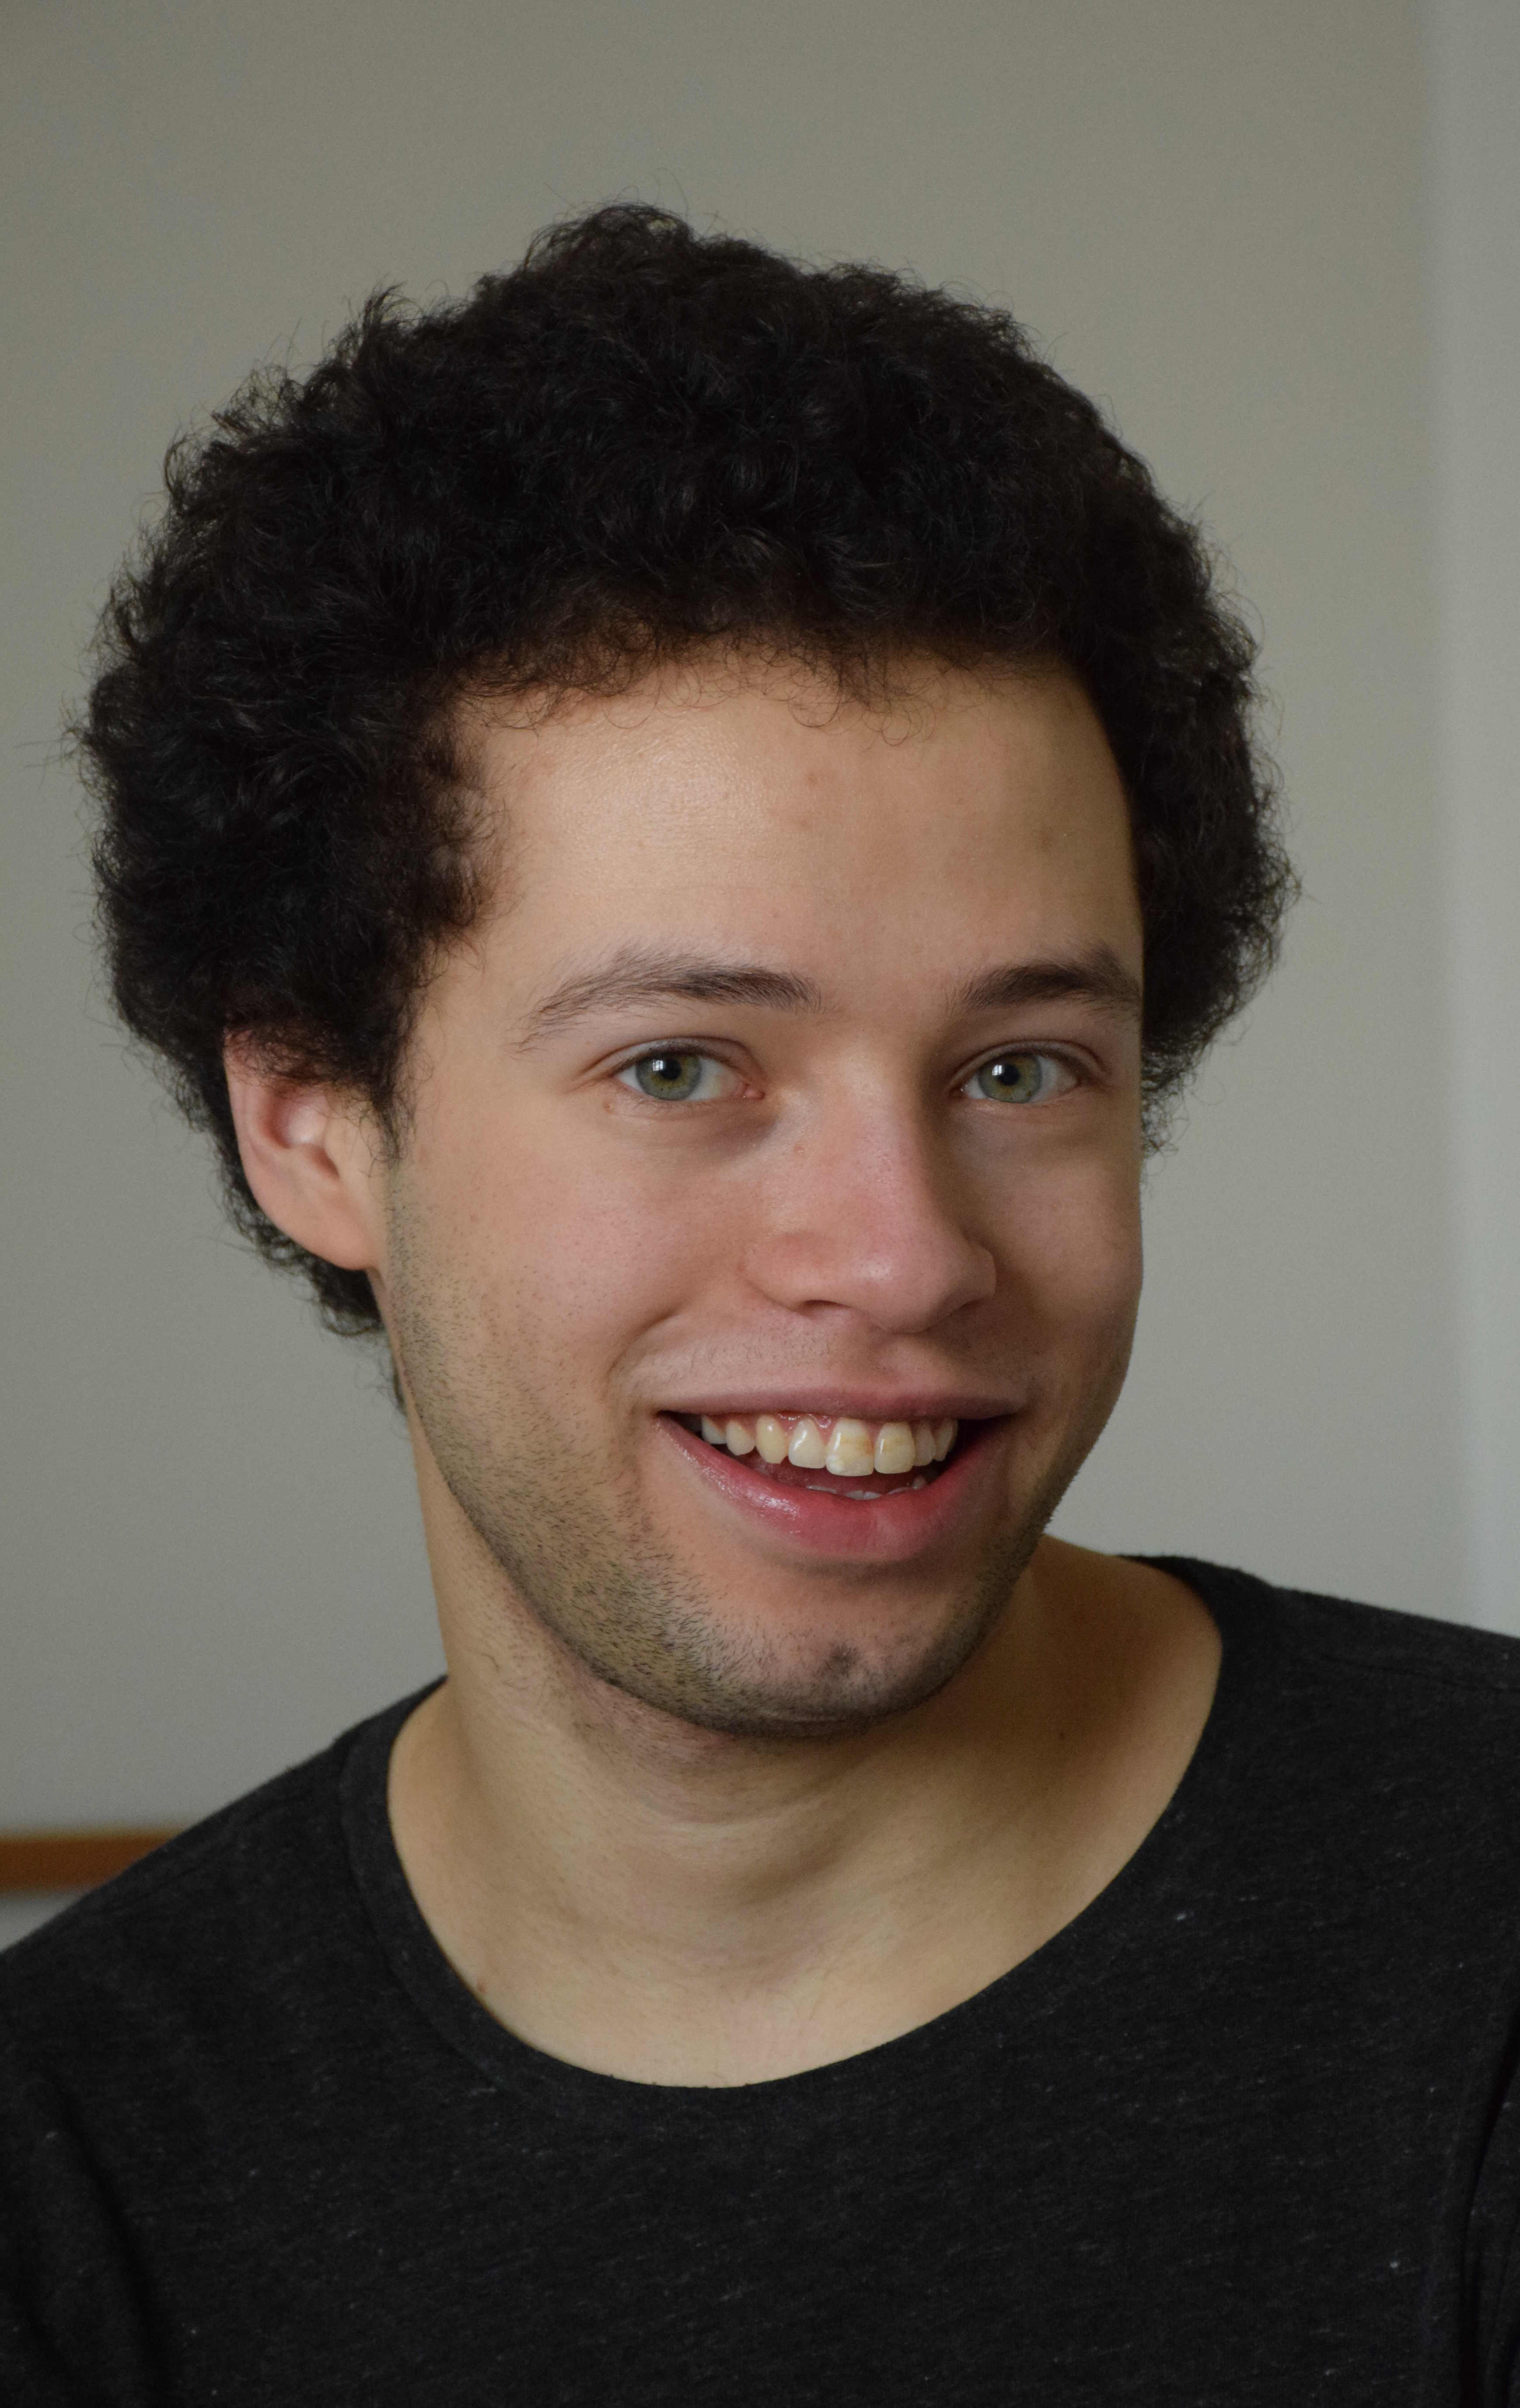
\includegraphics[width=3cm]{bild.jpeg}\\[\bigskipamount]
	% TODO hitta en bättre bild
}
\posttitle{\end{center}}
\title{
\huge{CV -- Malcolm Vigren}\vspace{-3ex}}
\date{\today}
\begin{document}
	\maketitle
\underline{Malcolm} John Shubi Vigren, 19950127--0970

Tallholmsvägen 91

589 37 Linköping

E-post: \underline{malcolm.vigren\at{}gmail.com}

Mobil: 0793 35 41 48

LinkedIn: \url{https://www.linkedin.com/in/malcolm-vigren/}

\section*{Arbetslivserfarenhet}
\begin{longtable}{@{}l p{13cm}}
\textbf{2020 - } & Feature-ingenjör på Veoneer (nu Arriver sedan april 2021).
    Samma roll som jag hade
    när jag arbetade som Attentec-konsult på företaget. \\

\textbf{2019 - 2020} & Konsult på Attentec AB. Började med att utveckla en portal
    för programmeringsprov för rekryteringssyften, med Angular och
    flask. Från januari 2020 har jag haft ett uppdrag på Veoneer, på
    avdelningen Road, med arbetsuppgifter som utveckling i C i en embeddedmiljö, C\#
    och Python, samt arbete med bildbehandling, testning och kravhantering. \\

\textbf{2019} & Examensarbete vid Veoneer i Linköping, där
    körfältsestimering skulle genomföras med deep learning, som kan hittas här:
    \url{http://urn.kb.se/resolve?urn=urn:nbn:se:liu:diva-157645}. \\

\textbf{2018} & Labbassistent och seminarieledare på hösten i \textit{Funktionell och
    imperativ programmering i Python} (TDDE23/24) på Linköpings
    Universitet. \\

\textbf{2018} & Extrajobb och sommarjobb på Veoneer i Linköping, från april till augusti.
    Arbetade i teamet ansvarig för datahantering på avdelningen
    Simulation. Arbetsuppgifter inkluderade utveckling i Python, JavaScript och
    C\#, testning, datahantering och signalbehandling. \\

\textbf{2017} & Labbassistent och seminarieledare på hösten i \textit{Funktionell och
    imperativ programmering i Python} (TDDE23/24) på Linköpings
    Universitet. \\

\textbf{2017} & Sommarjobb på Autoliv (nuvarande Veoneer/Arriver) i Linköping.
    Utvecklade verktyg för behandling av data och lagra dessa i en databas
    i C\# och Microsoft SQL Server. \\

\textbf{2016} & Sommarjobb på Autoliv (nuvarande Veoneer/Arriver) i Linköping.
    Utvecklade verktyg för utförande av regressionstester i Python och C\#.\\

\textbf{2015 - 2016} & Butiksarbetare på ICA Supermarket Eneby i Norrköping, med
arbetsuppgifter som kassör, spelombudsbiträde och postombudsbiträde, vid sidan
av universitetsstudier. \\

\textbf{2013} & Skapade en animerad film åt SundaHus för en mässa.
\\

\textbf{2012 - 2015} & Butiksarbetare på Hemköp Ljungsbrohallen,
med arbetsuppgifter
som kassör,
spelombudsbiträde, postombudsbiträde, ansvarig för ändring av priser med mera.
\\

\end{longtable}

\section*{Utbildning}
\begin{tabular}{@{}l p{11cm}}
	\textbf{Högskola} & \textit{Linköpings Universitet} - Civilingenjör i
	datateknik 300hp - Avslutad, examen juni 2019 \\

	\textbf{Gymnasieskola} & \textit{Berzeliusskolan} - Teknikvetenskap -
	Avslutad, examen 2014 \\

	\textbf{Grundskola} & \textit{Internationella Engelska Skolan i Linköping},
	årskurs 6-9 \\

	\textbf{Grundskola} & \textit{Brunnbyskolan}, årskurs 1-5 \\
\end{tabular}

\section*{Programmeringskunskaper}
Mycket goda kunskaper inom C, C\#, C++, Java, Python, Matlab och JavaScript.
Goda kunskaper inom Rust, Elm, TypeScript och assembler.
Grundläggande kunskaper inom ASP.NET, HTML, VHDL, Haskell, BASH-skript,
CoffeeScript och Ruby On Rails.

Goda kunskaper inom Git, VIM, LaTeX och Deep Learning-biblioteken PyTorch och
Keras. Erfarenhet av arbete i Gerrit, Jenkins, Jira, GitLab och DOORS.

Goda kunskaper inom bildbehandling, datorseende och deep learning.

\section*{Språkkunskaper}
Flytande svenska och engelska i tal och skrift. Gymnasiekunskaper inom tyska
(Tyska steg 3).

\section*{Profil och intressen}
Jag är systematisk, noggrann och lättlärd. Jag är engagerad i mitt arbete och
försöker alltid att göra mitt bästa. Mina huvudintressen är programmering, vetenskap,
teknik, matematik, datorer, motorer och bilar. Jag är musikintresserad och kan
spela trummor och piano.

\section*{Övriga meriter}
Körkort (AM- samt B-behörighet).

Erhöll 1000 kr ur Berzeliusskolans stipendiefond vid examen för mina höga
betyg.

Konstruerade och programmerade ett mekaniskt RGB-bakbelyst tangentbord som
hobbyprojekt under hösten 2016. Detta, och många andra av mina hobby- och skolprojekt, finns på min Github-sida: \url{https://github.com/malcx95}.

Var projektledare i projektarbetet under kursen \textit{Konstruktion med
mikrodatorer} (kurskod TSEA29) under höstterminen 2016.
I projektet skulle 7 projektmedlemmar
konstruera en sexbent robot, med en tidsbudget på 160 timmar per person. Koden
och dokumentationen för projektet finns på Github:
\url{https://github.com/TheZoq2/LiTHe-Hex}.

\end{document}
